\documentclass{article}
\usepackage[utf8]{inputenc}
\usepackage{amsmath}
\usepackage{amssymb}
\usepackage{amsfonts}
\usepackage[margin=1in,headheight=13.6pt]{geometry}
\usepackage{amsthm}
\theoremstyle{definition}
\newtheorem{definition}{Definition}[section]
\usepackage{graphicx}
\renewcommand{\baselinestretch}{1.5}
\usepackage{color}  
\usepackage{hyperref}
\hypersetup{
    colorlinks=true
    linktoc=all
    linkcolor=blue
}
\usepackage{tikz}
\usetikzlibrary{shapes,arrows}
\usepackage{fancyheadings}
\pagestyle{fancyplain}
\fancypagestyle{plain}{
\renewcommand{\headrulewidth}{0.4pt}
}
\lhead{\fancyplain{Heather Tan}{Heather Tan}}
\rhead{\fancyplain{An Introduction to Mediation Model}{An Introduction to Mediation Model}}
\title{An Introduction to Mediation Model}
\author{Heather Tan}
\date{July 2019}

\tikzset{
    vertex/.style = {
        circle,
        fill            = black,
        outer sep = 2pt,
        inner sep = 1pt,
    }
}
\tikzstyle{arrow} = [thick,->,>=stealth]
\begin{document}

\maketitle	
\tableofcontents
\pagebreak

\textbf{Simple mediation model} is used to introduce the mechanics of path analysis and to demonstrate how a variable's effect on an outcome can be partitioned into direct and indirect effects which are easily quantified using OLS regression.\\
Whereas answering questions about \textit{when} or \textit{for whom} are the domain of moderation analysis. Questions that ask about \textit{how} pertain to \textit{mediation}.

\section{The Simple Mediation Model}
\begin{center}
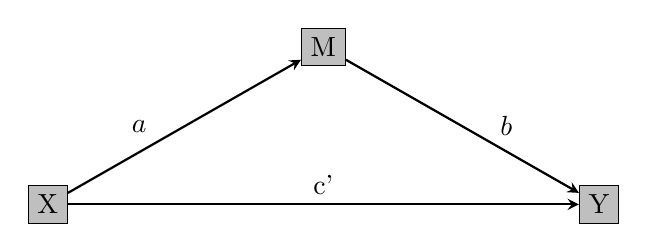
\begin{tikzpicture}
  \node[draw,fill = lightgray] (x) at (4,0) {X};
  \node[draw,fill = lightgray] (y) at (11,0) {Y};
  \node[draw,fill = lightgray] (m) at (7.5,2) {M};
 \draw [arrow] (x) -- node[anchor= south] {c'} (y);
 \draw [arrow] (x) -- node[anchor= east] {$a\quad$} (m);
 \draw [arrow] (m) -- node[anchor= west] {$\quad b$} (y);
\end{tikzpicture}\\
\textbf{Figure:A statistical diagram of a simple mediation model}	
\end{center}
This model contains two consequent variables M and Y, and two antecedent variables X and M, with X casually influencing Y and M, and M casually influencing Y.\\
\textbf{Direct Effect:} pathway leads from X to Y without passing through M.\\
\textbf{Indirect Effect: }pathway from X to Y through M.\\
\textbf{Mediator Variable: }M\\
Applied area: social psychology, cognitive, health, politics, medical sci, educational, communication, business literatures.\\
\textbf{Assumption: }It is assumed that the relationships in the system are casual, and M is usually located betweeen X and Y. M cannot possibly carry X's effect on Y if M is not located causally between X and Y.

\section{Estimation of the Direct, Indirect, and Total Effect of X}
As there are two consequent variables in this diagram, two linear models are required, one of each consequent.
\begin{equation*}
	M = i_1+aX+e_M\\
	Y = i_2+c'X+bM+e_Y
\end{equation*}
\textbf{Coefficients}
\begin{itemize}
	\item $1_1,i_2$ are regression intercepts
	\item $e_M, e_Y$ are errors in estimation of M and Y
	\item $q,b,c'$ are the regression coefficients of the antecedent variables i the model in the estimation of the consequents. These coefficients can be estimated by conducting two OLS regression analyses.
\end{itemize}

\subsection{The Direct Effect of X on Y(c')}
\textbf{Interpretation of Direct Effect: }two cases that differ by one unit on X, but are equal on M, are estimated to differ by c' units o Y. Formally
\begin{equation*}
	c' = [\hat{Y}| (X=x,M=m)]-[\hat{Y}| (X=x-1,M=m)]
\end{equation*}
The sign of c' tells whether the case one unit higher on X is estimated to be higher(c' = +) or lower(c' = -) on Y. \\
\textbf{(c' = +): }higher on X is estimated to be higher on Y.\\
\textbf{(c' = -): }higher on X is estimated to be lower on Y.\\
Since $\hat{Y}$ can be interpreted as a group mean, so $c' = [\bar{Y}| (X=x,M=m)]-[\bar{Y}| (X=x-1,M=m)]$, meaning c' estimates the difference between the two groups means holding M constant.\textbf{This is equivalent} to what in analysis of covariance terms is called \textbf{adjusted mean difference}

\subsection{The Indirect Effect(a,b) of X on Y}
In this model,\textbf{a} quantifies how much two cases that differ by on unit on X are estimated to differ on M, with the same sigh determination with c'
\begin{equation*}
 	a = [\hat{M}|(X=x)]-[\hat{M}|(X=x-1)]
\end{equation*}
In the statistical model $a = [\bar{M}|(X=x)]-[\bar{M}|(X=x-1)]$\\
The \textbf{b} coefficient in the statistical model has an interpretation analogous to c', except when M as the antecedent(antecedent i.e consider M as X that has direct effect on Y). Two cases that differ by one unit on M but that are equal on X are estimated to differ by b units on Y(i.e M's direct effect on Y).\\
\textbf{The indirect effect of X on Y through M is the product of a and b.} i.e The  indirect effect tells us that two cases that differ by one unit on X are estimated to differ by ab units on Y as a result of the effect of X on M which, in turn, affects Y
\subsection{The Total Effect of X on Y}
Total effect (denote as c) quantifies how much two cases that differ by one unit on X are estimated to differ on Y. That is 
\begin{equation*}
	c = [\hat{Y}| (X=x)] - [\hat{Y}|(X=x-1)]
\end{equation*}
In a simple mediation model, c can be derived by estimating Y from X alone
\begin{equation*}
	Y = i_3+cX+e_Y
\end{equation*}
The total effect of X on Y is equal to the sum of the direct and indirect effect of X
\begin{equation*}
	c = c'+ab
\end{equation*}
The indirect effect is the difference between the total effect of X on Y and the effect of X on Y controlling for M, the direct effect.Thereby expressing Y as a function of only X:
\begin{equation*}
	Y = i_2+b(i_1+aX+e_M)+c'X+e_Y = (i_2+bi_1) + (ab + c')X + (e_Y+be_M)
\end{equation*}
\subsection{Sample Analysis}
In a simple mediation model such as this, the total effect of X can be estimated merely by regressing Y on X alone, without M in the model.\\
The function of Total effect(c) = Direct effect(c') + Indirect effect(ab) can be rewritten as :
\begin{equation*}
	(\bar{Y}_{X=1} - \bar{Y}_{X=0}) = (\bar{Y}_{X=1}^* - \bar{Y}_{X=0}^*) + (\bar{M}_{X=1} - \bar{M}_{X=0})b
\end{equation*}

\section{Statistical Inference}
The effect of X on Y in a simple mediation model can be partitioned into direct and indirect components. When these effects are estimated using OLS regression, it will always be true in any data set that you can find, collect or imaging that c = c'+ab \\
However $c, c'$, and ab are sample specific instantiations of their true values $_Tc, _Tc',$ and $_Ta_Tb$.

\subsection{Inference about the Direct Effect of X on Y}
The direct effect quantifies the estimated difference in Y between two cases that differ by one unit on X independent of M's influence on Y.\\
Using the standard method used for inference for any regression coefficient in a regression model.\\
\textbf{Claim: }$_Tc$ is different from zero is justified based on the data available.i.e whether the coefficient of the direct effect is significant\\
\textbf{If so:} X is related to Y independent of the mechanism represented by M.\\
\textbf{If not: }There is no evidence of association between X and Y when the mechanism through M is accounted for.i.e X does not affect Y independent of M's effect on Y.\\
\textbf{Hypothetical Test: } $H_0: _Tc'=0$, $H_a:_Tc' \neq 0$ in order to determine whether an interval estimate for $_Tc'$ includes zero. 

\subsection{Inference about the Indirect Effect of X on Y through M}
The indirect effect is relevant as to whether X's effect on Y can be said to be transmitted through the mechanism represented by the X $\rightarrow $ M $\rightarrow$ Y causal chain of events. \\
\textbf{Claim: }whether the data allow for the claim that this estimated difference in Y attributable to this mechanism can be said to be different from zero.i.e whether the change of Y under this mechanism is significant.\\
\textbf{If so: } M can be claimed that it is served as a mediator of the effect of X on Y.

\subsubsection{The Normal Theory Approach}
A.k.a the product of coefficients approach to inference, the delta method or the Sobel Test. The indirect effect ab is a sample-specific instantiation of $_Ta_Tb$ which is subject to sampling variance.\\
\textbf{First-order delta estimator of the standard error}
\begin{equation*}
	se_{ab} = \sqrt{a^2se_b^2+b^2se_a^2}
\end{equation*}
\textbf{Second-order delta estimator of the standard error}
\begin{equation*}
	se_{ab} = \sqrt{a^2se_b^2+b^2se_a^2+se_a^2se_b^2}
\end{equation*}
With an estimate of the standard error of the direct effect, $H_0: _Ta_Tb = 0, H_a: _Ta_Tb \neq 0$, and then calculate z score as $z = \frac{ab}{se_{ab}}$ and find the related p-value. With the z score we can get CI as well:
\begin{equation*}
	CI: ab-Z_{\alpha \% se_{ab}} \leq _Ta_Tb \leq ab + Z_{\alpha \%}se_{ab}
\end{equation*}
\textbf{Disadvantage: }there is an assumption that is made about the shape of the sampling distribution of the indirect effect over repeated sampling from the population.

\subsubsection{Bootstrap Confidence Intervals}
Observations in this sample are then resampled with replacement, and some statistic of interest is calculated in the new sample of size n constructed through this resampling process. \\
In mediation analysis, bootstrapping is used to generate a representation of the sampling distribution of the indirect effect, and this representation is used for the construction of a confidence interval for $_Ta_Tb$\\
\textbf{Advantages: }
\begin{enumerate}
	\item have better representation about the variable distribution of the population
	\item better represented for smaller samples
	\item each time of the bootstrap would give slightly different confidence interval.
\end{enumerate}
A bootstrap confidence interval is called a percentile bootstrap confidence interval.

\section{Fundamentals of Moderation Analysis}
A moderation analysis is used to determine whether a certain variable influences or is related to the size of one variable's effect on another. Moderation a.k.a moderation.\\
\textbf{Moderation: }The effect of X on some variable Y is moderated by M if its size, sign, or strength depends on or can be predicted by M. \\
(The rest of the ideas about interaction can be found in the notes of STA302)


\end{document}